\section*{Electricity}
\label{sec:electricity}
\addcontentsline{toc}{section}{\nameref{sec:electricity}}

\subsection{General}

The preprocessed data was passed to the aforementioned set of algorithms in order to determine the best possible set of candidate predictors with some additional adjustments.  Only buildings that indicated electricity being used \lstinline{ELUSED} were included in the samples for this major fuel use.  Then, one of each pair of predictors with correlations above 0.75 were removed, to avoid model selection issues. Additionally, the other major fuel consumption values were removed from the set of possible predictors.  Also, the numeric predictors were transformed via BoxCox methodology as well as centered and scaled due to the varying scales and skewness.

Two potential outlier was found in the analysis. A public assembly space reported an energy consumption of 1E09 BTUs whereas the next highest consumption for this budiding type, with similar area was 3E08 BTU (less than one third of the value), and the 3rd quartile value of this subset is 5.5E06.  While it is noted that there were significantly higher indications of refrigeration use than other comparables, the inclusion of this data point still vastly skews most models due to its high leverage.  Similarly, an 'Other' space type has a reported energy consumption of 7E08 BTU whereas the next highest value is 2E08 BTU and the third quartile value is 2E06.  While this building is large (1.4 mmSF), and has a lot of server equipment (>500), it is still greatly beyond the next closest category and seems to be causing instability in the models due to lack of similar data points.  Therefore, these points have been removed and the caveat of instabilitity past a maximum limit will be instituted (>5E08 BTU), due to lack of additional information.

\subsection{Response Analysis}

The response data appear to be unimodal and have a heavy right skew.  After filtering for this model's end-use, there are 6499 samples in the data set.  The energy use was convert to units mmBTU (1e6 BTU) and the log was taken in an attempt to maintain homoscedacity as the variance of the energy used also scales with the magnitude.  \textit{\hyperref[appendix:electricity:response]{Appendix}}

\subsection{Variable Selection - PCA}
RMSE: NA, Rsquared: NA\\
Top 5: \lstinline{COOK.2[NO]}, \lstinline{LAUNDR..1[NA]}, \lstinline{ELCPLT..1[NA]}, \lstinline{PBA.14[EDUCATION]}, \lstinline{BLDPLT.2[NO]}
\\[0.1in]
\indent The principle component analysis indicates that only About 5.0\% of the variance in the data can be explained in the first principle component, which then drops to about 2\% for the second principle component.  These results reveal that there does not appear to be a clear set of axes that can explain the variance of the data very well, which indicates there may be some very complex interactions taking place in the predictors.  \textit{\hyperref[appendix:electricity:pca]{Appendix}}

\subsection{Variable Selection - PLS}
RMSE: 46880, Rsquared: 0.0.548\\
Top 5: \lstinline{NWKERPerSf}, \lstinline{RGSTRNPerSf}, \lstinline{FDSEATPerSf}, \lstinline{RFGWINPerSf}, \lstinline{PCTERMNPerSf}
\\[0.1in]
\indent This model returned a promising result; however, it must be noted that all predictors were used in this process.  Looking at the output thus far, it is appears that the number of workers, receptical equipment, and refrigeration equipment, influence electrical consumption.  \textit{\hyperref[appendix:electricity:pls]{Appendix}}

\subsection{Variable Selection - Random Forest}
RMSE: 163434, Rsquared: 0.173\\
Top 5: \lstinline{RFGWINPerSf}, \lstinline{RGSTRNPerSf}, \lstinline{NWKERPerSf}, \lstinline{RFGICNPerSf},  \lstinline{PCTERMNPerSf}
\\[0.1in]
\indent The resulting error metrics were much less promising.  However, similarly selected variables are are picked for this model when compared to the PLS.  \textit{\hyperref[appendix:electricity:rf]{Appendix}}

\subsection{Variable Selection - Lasso}
RMSE: NA, Rsquared: NA\\
 Top 5: NA
\\[0.1in]
\indent This resulted in a very poor fit, which is not unexpected.  Lasso models typically work when a few variables can be used to predict the response, which does not appear to be the case in this instance.  Due to the lack of fit, this model will not be used in the variable selection process.  Additionally, the actual model was poor enough that predictions could not be made on the data, which is the reason for the lack of reported metrics.

\subsection{Variable Selection - Forward Selection}
RMSE: 90503, Rsquared: 0.315\\
Top 5: \lstinline{NWKERPerSf}, \lstinline{RFGWINPerSf}, \lstinline{RFGWI.1[YES]}, \lstinline{RFGICNPerSf}, \lstinline{PCTERMNPerSf}
\\[0.1in]
\indent This model was building using the leaps package which iteratively selected the best predictor variable up to a limit of 100.  Unsurprisingly, the best model turned out to be the maximum setting.  Large refrigeration equipment load and typical office space attributes dominated this analysis, as appears to be the case in previous models.  It seems that in order to capture energy use for all buidling types, much more than 5 variables will be necessary.  \textit{\hyperref[appendix:electricity:lp]{Appendix}}

\subsection{Variable Selection - Recursive Feature Elimination}
RMSE: 48022, Rsquared: 0.517\\
Top 5: \lstinline{RGSTRNPerSf}, \lstinline{RFGICNPerSf}, \lstinline{NWKERPerSf}, \lstinline{PBAPLUS.32[FAST FOOD]}, \lstinline{RFGWINPerSf}
\\[0.1in]
\indent A more direct approach was taken with this model, which is specifically used to extract useful features from data sets. \textit{\hyperref[appendix:electricity:rfe]{Appendix}}

\subsection{Variable Selection - Simple Neural Network}
RMSE: 48644, Rsquared: 0.499\\
Top 5: \lstinline{FDSeatPerSf}, \lstinline{PBAPLUS.32[FAST FOOD]}, \lstinline{RFGWINPerSf}, \lstinline{RFGWI.1[YES]}, \lstinline{RGSTRNPerSf}
\\[0.1in]
\indent Given that the final model will be a neural network, it made sense to try a simple out-of-the-box training model to see if any particular features work better with this process.  As can be seen, there are some new attributes that surface which were not indicated to be of high importance previously.  \textit{\hyperref[appendix:electricity:snn]{Appendix}}
\newpage
\subsection{Variable Selection - Selected Variable Analysis}
\begin{figure}[h]
\begin{subfigure}{1\textwidth}
\centering
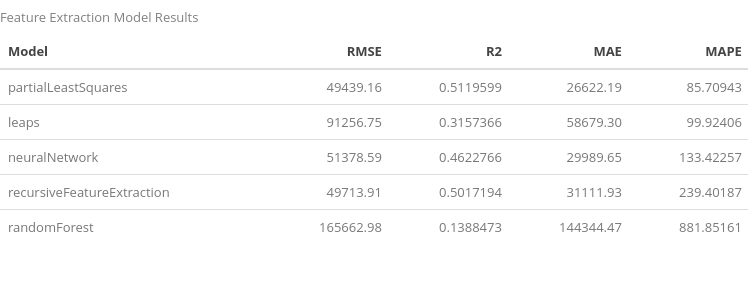
\includegraphics[width=.6\textwidth, height=0.2\textheight]{Images/electricity_psf_fe_summary.png}
\end{subfigure}
\begin{subfigure}{1\textwidth}
\centering
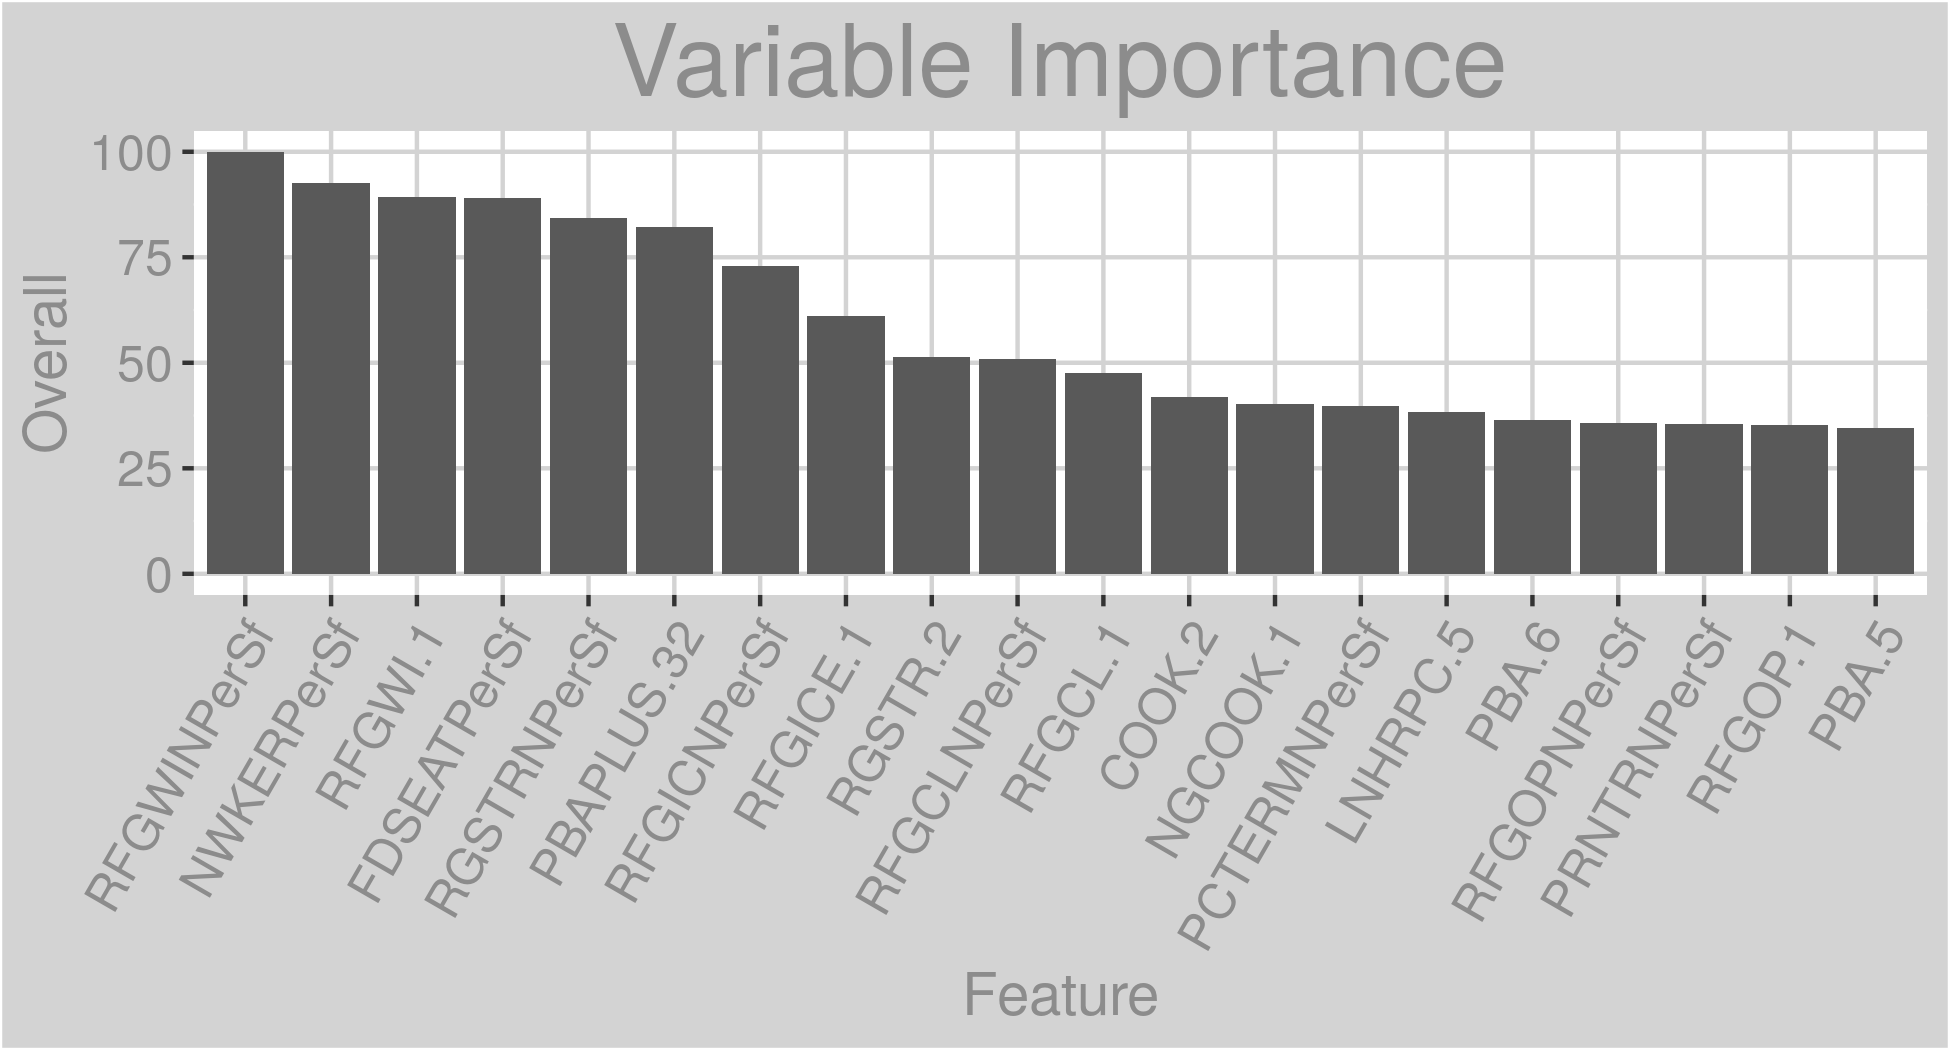
\includegraphics[width=.99\textwidth, height=0.3\textheight]{Images/electricity_psf_all_vars.png}
\end{subfigure}
\end{figure}
In order to rank the most impactful features, the variable importance metrics from the selected models were all set to the same scale then summed up.  As a preliminary check, the top 20 predictors are plotted in the appendix and are generally discussed here.  It seems the attempts to create stratified random samples may have been beneficial in this case since there are some building type specific end-uses that are highly ranked.  As previously noted, there are many attributes associated with refrigeration, office, and food sales equipment.  Also, the attribute identifying one of the more atypical building types, speaking in an energy intensity sense, has made it into the top 20 (\lstinline{PBA.5[NON-REFRIGERATED WAREHOUSE]}).  Additionally, some occupancy features (\lstinline{NWKERPerSf}, \lstinline{FDSEATPerSf}) have been included which is expected given that they impact interior space cooling and ventilation loads. In an attempt to truly follow the imporant predictors, no variables have been removed from this set and the order of importance remains unchanged.  \textit{\hyperref[appendix:electricity:sva]{Appendix}}